
\section{Challenges in LLM-Generated Code Detection}
\label{sec:Challenges in LLM-Generated Code Detection}
The detection of short texts generated by LLMs remains 
a challenging task. While partial solutions have been 
proposed, the problem cannot yet be considered fully 
resolved. Nonetheless, it is widely acknowledged that 
detection tools achieve strong performance when applied 
to moderately sized texts (longer than just a few lines).

A well-known example is \textbf{DetectGPT}
\cite{mitchell2023detectgpt}, a 
zero-shot method that does not require training a 
separate classifier but instead relies on an 
auxiliary LLM to assess whether a given passage is 
likely machine-generated. 
DetectGPT is often regarded as the state-of-the-art 
among open-source methods for AI-generated text detection.

%Eliminato per rientrare in una pagina
%However, recent studies have shown that even minimal 
%perturbations to LLM-generated outputs can significantly 
%reduce detection AUROC, in some cases down to 
%42\% \cite{krishna2023paraphrasing}. These findings 
%highlight that detection performance is highly 
%sensitive to surface-level edits.

In addition to open-source methods, commercial 
solutions such as \textbf{GPTZero} \cite{GPTZeroMethodology2023}
have gained 
popularity. GPTZero can be accessed via a web 
interface and combines language-model-based heuristics 
with machine learning classifiers. While it is 
effective in many cases, it is not infallible. 
For example, GPTZero has been reported to mistakenly 
flag texts written by non-native speakers, 
whose lexical variety may be lower, as AI-generated.

Even the creators of GPTZero explicitly state 
that a positive detection should not be taken as 
conclusive proof, but rather as a probabilistic 
signal or indicator.

\vspace{1\baselineskip}
\noindent

As stated in several papers analysed in this work, 
such as \textit{Uncovering LLM-Generated Code: A 
Zero-Shot Synthetic Code Detector via Code Rewriting 
\cite{ye2023uncovering}}, \textbf{methods designed for 
detecting natural language text are largely 
ineffective when applied to code}. The causes of 
this limitation are primarily related to the 
structural and syntactic properties of programming 
languages. 

Unlike natural language, where the same idea 
can be expressed using a vast variety of words 
and syntactic structures, source code is governed 
by strict and formal grammar rules. As a result, 
many tokens must appear in a specific and rigid 
order. Consequently, techniques based on lexical 
probability, such as those used by DetectGPT, 
tend to fail when applied to code, as they cannot 
meaningfully capture the constrained nature of 
programming syntax.

Moreover, many natural language detectors 
rely on input perturbation to assess sensitivity 
or likelihood distributions, a process that is 
significantly more difficult to perform on source 
code without introducing semantic or syntactic errors.

A further practical limitation is the lack of 
publicly available datasets specifically designed 
for training code-based LLM detectors. While large 
and well-established code corpora do exist, 
researchers who aim to train classification models 
for code detection often have to construct their 
own datasets, with all the associated challenges 
in terms of bias, coverage, and quality assurance.

These issues have contributed to a significant 
gap in the literature: unlike DetectGPT, which is 
widely recognized for natural language detection, 
there is no single, consolidated approach for 
LLM-generated code detection. Instead, the field 
is characterized by a proliferation of parallel 
methods, often employing fundamentally different 
techniques and evaluation protocols.



%\begin{figure}[H]
%    \centering
%    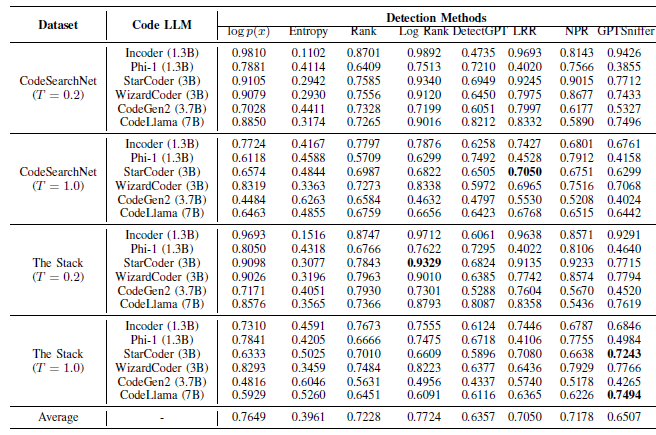
\includegraphics[width=0.9\textwidth]{img/1/Berween.png}
%    \caption{Performance (AUROC) of various detection methods from \cite{shi2024between}.}
%    \label{fig:Performance (AUROC) of various detection methods}
%\end{figure}